

\tikzset{every picture/.style={line width=0.75pt}} %set default line width to 0.75pt        

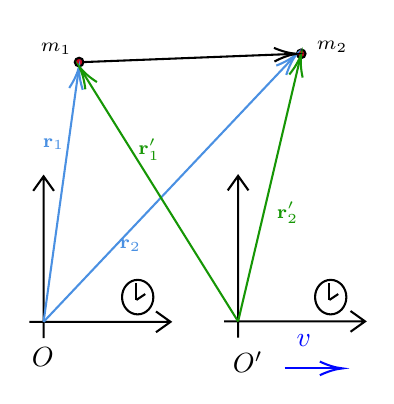
\begin{tikzpicture}[x=0.75pt,y=0.75pt,yscale=-1,xscale=1]
%uncomment if require: \path (0,186); %set diagram left start at 0, and has height of 186

%Shape: Axis 2D [id:dp22236225290792944] 
\draw  (225,146.23) -- (292.96,146.23)(231.8,76.12) -- (231.8,154.02) (285.96,141.23) -- (292.96,146.23) -- (285.96,151.23) (226.8,83.12) -- (231.8,76.12) -- (236.8,83.12)  ;
%Shape: Axis 2D [id:dp027564847074658116] 
\draw  (318.73,146.01) -- (386.68,146.01)(325.52,75.9) -- (325.52,153.8) (379.68,141.01) -- (386.68,146.01) -- (379.68,151.01) (320.52,82.9) -- (325.52,75.9) -- (330.52,82.9)  ;
%Straight Lines [id:da8338287582907346] 
\draw [color={rgb, 255:red, 0; green, 6; blue, 255 }  ,draw opacity=1 ]   (347.98,168.65) -- (373.84,168.65) ;
\draw [shift={(375.84,168.65)}, rotate = 180] [color={rgb, 255:red, 0; green, 6; blue, 255 }  ,draw opacity=1 ][line width=0.75]    (10.93,-3.29) .. controls (6.95,-1.4) and (3.31,-0.3) .. (0,0) .. controls (3.31,0.3) and (6.95,1.4) .. (10.93,3.29)   ;
%Shape: Circle [id:dp5997377273143482] 
\draw  [fill={rgb, 255:red, 208; green, 2; blue, 27 }  ,fill opacity=1 ] (353.83,17.08) .. controls (353.83,15.93) and (354.77,15) .. (355.92,15) .. controls (357.07,15) and (358,15.93) .. (358,17.08) .. controls (358,18.23) and (357.07,19.17) .. (355.92,19.17) .. controls (354.77,19.17) and (353.83,18.23) .. (353.83,17.08) -- cycle ;
%Straight Lines [id:da42368451729998724] 
\draw [color={rgb, 255:red, 74; green, 144; blue, 226 }  ,draw opacity=1 ]   (231.8,146.23) -- (352.46,18.54) ;
\draw [shift={(353.83,17.08)}, rotate = 133.38] [color={rgb, 255:red, 74; green, 144; blue, 226 }  ,draw opacity=1 ][line width=0.75]    (10.93,-3.29) .. controls (6.95,-1.4) and (3.31,-0.3) .. (0,0) .. controls (3.31,0.3) and (6.95,1.4) .. (10.93,3.29)   ;
%Straight Lines [id:da4528896382478149] 
\draw [color={rgb, 255:red, 22; green, 150; blue, 5 }  ,draw opacity=1 ]   (325.52,146.01) -- (355.46,19.11) ;
\draw [shift={(355.92,17.17)}, rotate = 103.27] [color={rgb, 255:red, 22; green, 150; blue, 5 }  ,draw opacity=1 ][line width=0.75]    (10.93,-3.29) .. controls (6.95,-1.4) and (3.31,-0.3) .. (0,0) .. controls (3.31,0.3) and (6.95,1.4) .. (10.93,3.29)   ;
%Shape: Ellipse [id:dp7373920249939159] 
\draw   (362.6,134.32) .. controls (362.6,129.72) and (365.98,126) .. (370.14,126) .. controls (374.31,126) and (377.68,129.72) .. (377.68,134.32) .. controls (377.68,138.91) and (374.31,142.63) .. (370.14,142.63) .. controls (365.98,142.63) and (362.6,138.91) .. (362.6,134.32) -- cycle ;
%Straight Lines [id:da13585636112426425] 
\draw    (369.52,135.68) -- (373.78,132.83) ;
%Straight Lines [id:da466483733182827] 
\draw    (369.52,135.68) -- (369.52,127.36) ;
%Shape: Ellipse [id:dp5796455244824992] 
\draw   (269.6,134.32) .. controls (269.6,129.72) and (272.98,126) .. (277.14,126) .. controls (281.31,126) and (284.68,129.72) .. (284.68,134.32) .. controls (284.68,138.91) and (281.31,142.63) .. (277.14,142.63) .. controls (272.98,142.63) and (269.6,138.91) .. (269.6,134.32) -- cycle ;
%Straight Lines [id:da16432097861546346] 
\draw    (276.52,135.68) -- (280.78,132.83) ;
%Straight Lines [id:da6230756844563958] 
\draw    (276.52,135.68) -- (276.52,127.36) ;
%Shape: Circle [id:dp5886404336660293] 
\draw  [fill={rgb, 255:red, 208; green, 2; blue, 27 }  ,fill opacity=1 ] (246.83,21.08) .. controls (246.83,19.93) and (247.77,19) .. (248.92,19) .. controls (250.07,19) and (251,19.93) .. (251,21.08) .. controls (251,22.23) and (250.07,23.17) .. (248.92,23.17) .. controls (247.77,23.17) and (246.83,22.23) .. (246.83,21.08) -- cycle ;
%Straight Lines [id:da41554898317876876] 
\draw [color={rgb, 255:red, 74; green, 144; blue, 226 }  ,draw opacity=1 ]   (231.8,146.23) -- (248.64,25.15) ;
\draw [shift={(248.92,23.17)}, rotate = 97.92] [color={rgb, 255:red, 74; green, 144; blue, 226 }  ,draw opacity=1 ][line width=0.75]    (10.93,-3.29) .. controls (6.95,-1.4) and (3.31,-0.3) .. (0,0) .. controls (3.31,0.3) and (6.95,1.4) .. (10.93,3.29)   ;
%Straight Lines [id:da5793257422387672] 
\draw [color={rgb, 255:red, 22; green, 150; blue, 5 }  ,draw opacity=1 ]   (325.52,146.01) -- (249.97,24.86) ;
\draw [shift={(248.92,23.17)}, rotate = 58.05] [color={rgb, 255:red, 22; green, 150; blue, 5 }  ,draw opacity=1 ][line width=0.75]    (10.93,-3.29) .. controls (6.95,-1.4) and (3.31,-0.3) .. (0,0) .. controls (3.31,0.3) and (6.95,1.4) .. (10.93,3.29)   ;
%Straight Lines [id:da02793406591260661] 
\draw    (251,21.08) -- (351.83,17.16) ;
\draw [shift={(353.83,17.08)}, rotate = 177.77] [color={rgb, 255:red, 0; green, 0; blue, 0 }  ][line width=0.75]    (10.93,-3.29) .. controls (6.95,-1.4) and (3.31,-0.3) .. (0,0) .. controls (3.31,0.3) and (6.95,1.4) .. (10.93,3.29)   ;

% Text Node
\draw (352.23,151.08) node [anchor=north west][inner sep=0.75pt]  [color={rgb, 255:red, 0; green, 6; blue, 255 }  ,opacity=1 ]  {$v$};
% Text Node
\draw (224.64,157.22) node [anchor=north west][inner sep=0.75pt]    {$O$};
% Text Node
\draw (321.56,159.22) node [anchor=north west][inner sep=0.75pt]    {$O'$};
% Text Node
\draw (362,9.4) node [anchor=north west][inner sep=0.75pt]  [font=\scriptsize]  {$m_{2}$};
% Text Node
\draw (230,56.4) node [anchor=north west][inner sep=0.75pt]  [font=\scriptsize,color={rgb, 255:red, 74; green, 144; blue, 226 }  ,opacity=1 ]  {$\mathbf{r}_{1}$};
% Text Node
\draw (342.72,86.99) node [anchor=north west][inner sep=0.75pt]  [font=\scriptsize,color={rgb, 255:red, 22; green, 150; blue, 5 }  ,opacity=1 ]  {$\mathbf{r}_{2} '$};
% Text Node
\draw (229,10.4) node [anchor=north west][inner sep=0.75pt]  [font=\scriptsize]  {$m_{1}$};
% Text Node
\draw (267,105.4) node [anchor=north west][inner sep=0.75pt]  [font=\scriptsize,color={rgb, 255:red, 74; green, 144; blue, 226 }  ,opacity=1 ]  {$\mathbf{r}_{2}$};
% Text Node
\draw (276,56.4) node [anchor=north west][inner sep=0.75pt]  [font=\scriptsize,color={rgb, 255:red, 22; green, 150; blue, 5 }  ,opacity=1 ]  {$\mathbf{r}_{1} '$};
% Text Node
\draw (288,5) node [anchor=north west][inner sep=0.75pt]  [font=\scriptsize] [align=left] {$\rcurs$};


\end{tikzpicture}
